% !TeX root = ../Book1.tex
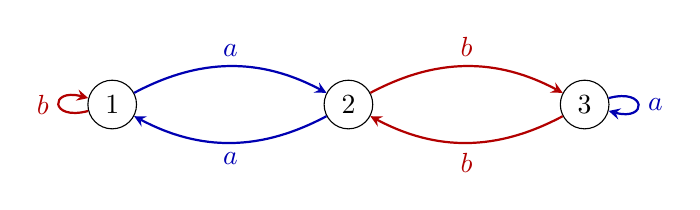
\begin{tikzpicture}[x=1cm,y=1cm,>=stealth]
	\node[circle,draw,minimum size=6mm] (v1) at (0,0) {\(1\)};
	\node[circle,draw,minimum size=6mm] (v2) at (3,0) {\(2\)};
	\node[circle,draw,minimum size=6mm] (v3) at (6,0) {\(3\)};
	\draw[blue!70!black,thick,->] (v1) to[bend left=28] node[above] {\(a\)} (v2);
	\draw[blue!70!black,thick,->] (v2) to[bend left=28] node[below] {\(a\)} (v1);
	\draw[red!70!black,thick,->] (v2) to[bend left=28] node[above] {\(b\)} (v3);
	\draw[red!70!black,thick,->] (v3) to[bend left=28] node[below] {\(b\)} (v2);
	\draw[red!70!black,thick,->] (v1) to[loop left] node[left] {\(b\)} (v1);
	\draw[blue!70!black,thick,->] (v3) to[loop right] node[right] {\(a\)} (v3);
\end{tikzpicture}
